
\documentclass[preprint2]{emulateapj}

\usepackage{natbib}
\bibliographystyle{apj}
\usepackage{longtable}
\usepackage[]{graphicx}
\usepackage{amsmath}
\usepackage{natbib}
\usepackage{tabularx}
\usepackage{bm}

%% Sometimes a paper's abstract is too long to fit on the
%% title page in preprint2 mode. When that is the case,
%% use the longabstract style option.

%% \documentclass[preprint2,longabstract]{aastex}

\newcommand{\vdag}{(v)^\dagger}
\newcommand{\myemail}{gsavorgn@astro.swin.edu.au}
\newcommand{\fitfigurewidth}{0.8\textwidth}


\shorttitle{M-M paper}
\shortauthors{Savorgnan et al.}

\begin{document}

\title{M-M paper, morphological bias }

\author{G. A. D. Savorgnan\altaffilmark{1} and A. W. Graham\altaffilmark{1}}
\affil{Centre for Astrophysics and Supercomputing, Swinburne University of Technology, Hawthorn, Victoria 3122, Australia.}
\email{gsavorgn@astro.swin.edu.au}

%\and

%\author{A. W. Graham\altaffilmark{1}}
%\affil{Centre for Astrophysics and Supercomputing, Swinburne University of Technology, Hawthorn, Victoria 3122, Australia.}

%% Notice that each of these authors has alternate affiliations, which
%% are identified by the \altaffilmark after each name.  Specify alternate
%% affiliation information with \altaffiltext, with one command per each
%% affiliation.

%\altaffiltext{1}{Visiting Astronomer, Cerro Tololo Inter-American Observatory.
%CTIO is operated by AURA, Inc.\ under contract to the National Science
%Foundation.}
%\altaffiltext{2}{Society of Fellows, Harvard University.}
%\altaffiltext{3}{present address: Center for Astrophysics,
%    60 Garden Street, Cambridge, MA 02138}
%\altaffiltext{4}{Visiting Programmer, Space Telescope Science Institute}
%\altaffiltext{5}{Patron, Alonso's Bar and Grill}

%% Mark off your abstract in the ``abstract'' environment. In the manuscript
%% style, abstract will output a Received/Accepted line after the
%% title and affiliation information. No date will appear since the author
%% does not have this information. The dates will be filled in by the
%% editorial office after submission.

\begin{abstract}
abstract 
\end{abstract}

\keywords{keywords}

\section{Introduction}
\label{sec:int}
More than two and a half decades ago, 
\cite{dressler1989} foresaw a ``rough scaling of black hole mass with the mass of the spheroidal component'', 
as suggested by the sequence of five galaxies (M87, M104, M31, M32 and the Milky Way). 
His ``rough scaling'' was a premature version of the nowadays popular correlation between black hole mass, $M_{\rm BH}$,  
and host spheroid luminosity, $L_{\rm sph}$, and also host spheroid mass, $M_{\rm sph}$ 
\citep{yee1992,kormendyrichstone1995,magorrian1998,marconihunt2003,haringrix2004}. 
These early studies were dominated by high-mass, early-type galaxies, 
for which they reported a quasi-linear $M_{\rm BH} - M_{\rm sph}$ relation, 
consistent with a dry-merging formation scenario. 
Subsequent studies of the $M_{\rm BH} - L_{\rm sph}$ and $M_{\rm BH} - M_{\rm sph}$ diagrams 
(\citealt{ferrareseford2005,lauer2007,graham2007,graham2008bar,gultelkin2009,sani2011,beifiori2012,erwingadotti2012,
vika2012,vandenbosch2012,mcconnellma2013,kormendyho2013,rusli2013}; 
see \citealt{graham2015bulges} for an extensive review about the early discovery and successive improvements of these correlations)
used similar galaxy samples, which remained dominated by high-mass, early-type objects having $M_{\rm BH} \gtrsim 0.5 \times 10^8~\rm M_\odot$, 
and recovered a near-linear relation. 
However, the consensus about a linear $M_{\rm BH} - M_{\rm sph}$ correlation was not unanimous. 
Some studies reported a slope steeper than one,  
or noticed that low-mass spheroids were downwards offset from the relation traced by their high-mass counterparts 
\citep{laor1998,wandel1999,laor2001,ryan2007}.
Recently, \cite{lasker2014data,lasker2014anal} derived $2.2~\rm \mu m$ bulge luminosities for 35 galaxies 
(among which only 4 were classified as spiral galaxies), 
and reported a slope below unity for their $M_{\rm BH} - M_{\rm sph}$ relation. 
They also claimed that the black hole mass correlates equally well with the total galaxy luminosity 
as it does with the bulge luminosity. \\
The $M_{\rm BH} - L_{\rm sph}$ relation can be predicted from other two correlations involving the bulge velocity dispersion, $\sigma$.
The first of these two is the $M_{\rm BH} - \sigma$ relation \citep{ferraresemerritt2000,gebhardt2000},
which can be described by a single power-law ($M_{\rm BH} \propto \sigma^5$) 
over the range in velocity dispersion $70-350~\rm km~s^{-1}$ (e.g.~\citealt{graham2011,mcconnell2011,grahamscott2013}).
The second is the $L_{\rm sph} - \sigma$ relation, 
which has long been known to be a ``double power-law'', 
being $L_{\rm sph} \propto \sigma^5$ at the luminous end \citep{schechter1980,malumuthkrishner1981,vonderlinden2007,liu2008}, 
and $L_{\rm sph} \propto \sigma^2$ at intermediate and faint luminosities 
\citep{davies1983,held1992,matkovicguzman2005,derijcke2005,balcells2007screl,chilingarian2008,forbes2008,cody2009,tortora2009,kourkchi2012}. 
The change in slope of the $L_{\rm sph} - \sigma$ relation occurs at $M_B \approx -20.5\rm~mag$, 
corresponding to $\sigma \approx 200~\rm km~s^{-1}$. 
That is, the $M_{\rm BH} - L_{\rm sph}$ relation should be better described by a ``broken'', rather than a single, power-law, 
having $M_{\rm BH} \propto L_{\rm sph}^{2.5}$ at the low-luminosity end, 
and $M_{\rm BH} \propto L_{\rm sph}^1$ at the high-luminosity end.  
Due to the scatter in the $M_{\rm BH} - L_{\rm sph}$ (or $M_{\rm BH} - M_{\rm sph}$) diagram, 
studies that have not sufficiently probed below $M_{\rm BH} \approx 10^7\rm~M_\odot$ 
can easily miss the change in slope occuring at $M_{\rm BH} \approx 10^{(8 \pm 1)}\rm~M_\odot$, 
and erroneously recover a single log-linear relation. \\
When \cite{graham2012bent} pointed out this overlooked inconsistency, 
he identified two different populations of galaxies, 
namely the core-S\'ersic \citep{graham2003coresersicmodel,trujillo2004coresersicmodel} and S\'ersic 
spheroids\footnote{Core-S\'ersic spheroids have partially depleted cores relative to their outer S\'ersic light profile, 
whereas S\'ersic spheroids have no central deficit of stars. 
While core-S\'ersic spheroids are also ``core galaxies'', as given by the Nuker definition \citep{lauer2007lumell},
it should be noted that $\sim$20\% of ``core galaxies'' are not core-S\'ersic spheroids 
(\citealt{dullograham2014cores}, their Appendix A.2), i.e. do not have depleted cores.
The change in slope of the $L_{\rm sph} - \sigma$ relation corresponds to the division between 
core-S\'ersic and S\'ersic spheroids (e.g. \citealt{grahamguzman2003}).},
and attributed the change in slope (from log-quadratic to log-linear) to their different formation mechanisms. 
In this scenario, core-S\'ersic spheroids are built in additive dry merger events, 
where the black hole and the bulge grow at the same pace, increasing their mass in lock steps ($M_{\rm BH} \propto L_{\rm sph}^1$), 
whereas S\'ersic spheroids originate from gas-rich processes, 
in which the mass of the black hole increases more rapidly than the mass of its host spheroid ($M_{\rm BH} \propto L_{\rm sph}^{2.5}$). 
\cite{grahamscott2013} and \cite{scott2013} presented double power-law linear regressions 
for S\'ersic/core-S\'ersic spheroids in the $M_{\rm BH} - L_{\rm sph}$ and $M_{\rm BH} - M_{\rm *,sph}$ 
(spheroid stellar mass) diagrams, respectively, probing down to $M_{\rm BH} \approx 10^6\rm~M_\odot$. 
To obtain their dust-corrected \emph{bulge} magnitudes, they did not perform bulge/disc decompositions, 
but instead they converted $B-$band and $K_S-$band observed, total \emph{galaxy} magnitudes 
using a mean statistical correction based on each object's morphological type and disc 
inclination\footnote{While this resulted in individual bulge magnitudes not being exactly correct, 
their large sample size allowed them to obtain a reasonably ensemble average correction.}. 
It should be noted that $\sim$80\% of their core-S\'ersic spheroids were morphologically classified as elliptical galaxies, 
and $\sim$80\% of their S\'ersic spheroids were morphologically classified as bulges of disk galaxies (lenticulars and spirals). \\
Several recent papers \citep{jiang2011a,jiang2013,mathur2012,reines2013} claimed an offset at the low-mass end of the $M_{\rm BH} - M_{\rm *,sph}$ diagram,
such that the black hole mass is lower than expected from the near-linear correlation traced by the high-mass, early-type spheroids. 
However, \cite{grahamscott2015} showed that the low-mass spheroids ($10^{8.5} \lesssim M_{\rm *,sph}/{\rm M_\odot} \lesssim 10^{10.5}$) 
are not randomly offset from the high-mass, near-linear correlation, 
but lie on the two times steeper relation traced by the S\'ersic spheroids. \\
Here we investigate substructure in the $M_{\rm BH} - L_{\rm sph}$ and $M_{\rm BH} - M_{\rm *,sph}$ diagrams 
using state-of-the-art galaxy decompositions (Savorgnan \& Graham \emph{in preparation}, hereafter \emph{Paper I}) 
for the largest sample of galaxies with directly measured black hole masses.
Our decompositions were obtained from $3.6\rm~\mu m$ \emph{Spitzer} satellite imagery, 
which is an excellent proxy for the stellar mass, superior to the $K-$band (\citealt{sheth2010} and references therein).
Nine of our galaxies have $M_{\rm BH} \lesssim 10^7\rm~M_\odot$, 
which allows us to accurately constrain the slope of the correlation at the low-mass end.
In addition to this, our galaxy sample includes 17 spiral galaxies, 
representing a notable improvement over the past studies dominated by early-type systems.




 

\section{Data}
\label{sec:data}
Our galaxy sample (see Table \ref{tab:sample}) 
consists of 66 objects for which a dynamical measurement of the black hole mass had been reported in the literature 
\citep{grahamscott2013,rusli2013bhmassesDM} at the time we started this project, 
and for which we were able to obtain useful bulge parameters from $3.6\rm~\mu m$ \emph{Spitzer} satellite imagery. 
Bulge magnitudes were derived from our state-of-the-art galaxy decompositions, which take into account 
bulges, disks, spiral arms, bars, rings, haloes, extended or unresolved nuclear sources and partially depleted cores.
Kinematical information \citep{atlas3dIII-MNRAS,scott2014,arnold2014} was used 
to confirm the presence of rotationally supported components in most early-type galaxies, 
and to identify their extent (intermediate-scale, embedded disks or large-scale disks). 
\emph{Paper I} will present the dataset used here to investigate the $M_{\rm BH} - L_{\rm sph}$ and $M_{\rm BH} - M_{\rm *,sph}$ diagrams, 
give details about the data reduction process and the sophisticated galaxy modelling technique that we developed, 
discuss how we estimated the uncertainties on the bulge parameters, 
and illustrate the individual 66 galaxy decompositions. \\
Bulge luminosities\footnote{Absolute luminosities were calculated assuming a $3.6\rm~\mu m$ solar absolute magnitude of $3.25\rm~mag$ \citep{sani2011}.} 
were converted into stellar masses using the colour-$\Gamma_{3.6}$ relation published by 
\citeauthor{meidt2014} (\citeyear{meidt2014}, their equation 4), 
which allows one to estimate the $3.6\rm~\mu m$ mass-to-light ratio, $\Gamma_{3.6}$, of a galaxy 
from its $[3.6] - [4.5]$ colour. 
Individual $[3.6] - [4.5]$ colours\footnote{These are integrated $[3.6] - [4.5]$ colours, measured in a circular aperture 
within one galaxy's effective radius.} were taken from 
\citeauthor{peletier2012} (\citeyear{peletier2012}, column 8 of their Table 1) 
when available for our galaxies, 
or were estimated from the bulge stellar velocity dispersion, $\sigma$, 
using the colour-$\sigma$ relation presented by \citeauthor{peletier2012} (\citeyear{peletier2012}, their Figure 6).
We point out here that using a single $\Gamma_{3.6} = 0.6$, independent of $[3.6] - [4.5]$ colour, 
does not significantly affect the results of our analysis. \\
The S\'ersic/core-S\'ersic classification presented in this work 
comes from the compilation of \citet{savorgnangraham2014},
who identified partially depleted cores according to the same criteria used by \citet{grahamscott2013}.
When no high-resolution image analysis was available from the literature, 
they inferred the presence of a partially depleted core based on the stellar velocity dispersion:
a galaxy is classified as core-S\'ersic if $\sigma > 270\rm~km~s^{-1}$,
or as S\'ersic if $\sigma < 166\rm~km~s^{-1}$. \\
For each galaxy, the total luminosity (or galaxy luminosity) is the sum of the luminosities of all its sub-components. 
Due to the complexity of their modelling, 
four galaxies (see Table \ref{tab:sample}, column 7) had their galaxy luminosities 
underestimated\footnote{These four cases will be discussed in \emph{Paper I}.}, 
which are given here as lower limits. 


\begin{table*}                                        
\begin{center}                                        
\caption{{\bf Galaxy sample.}                        
\emph{Column (1):} Galaxy name.                       
\emph{Column (2):} Distance.                                   
\emph{Column (3):} Black hole mass.                                   
\emph{Column (4):} Reference of the black hole mass reported here (G+03 = \citealt{greenhill2003}, GS13 = \citealt{grahamscott2013}; R+13b = \citealt{rusli2013bhmassesDM}).                                   
\emph{Column (5):} Presence of a partially depleted core. 
The question mark is used when the classification has come from the velocity dispersion criteria mentioned in Section \ref{sec:corser}. 
The value of the core break radius is reported in parenthesis when available.  
\emph{Column (6):} Reference of the identification of a partially depleted core (G+94 = \citealt{grillmair1994}; F+97 = \citealt{forbes1997}; Q+00 = \citealt{quillen2000}, 
T+04 = \citealt{trujillo2004coresersicmodel}; F+06 = \citealt{ferrarese2006acsvcs}; J+11 = \citealt{jardel2011}; R+11 = \citealt{richings2011}; 
DG13 = \citealt{dullograham2013cores}; R+13a = \citealt{rusli2013}).  
\emph{Column (7):} Kinematical classification (fast/slow rotator).
\emph{Column (8):} Availability of velocity map (A = ATLAS$^{\rm 3D}$, S = SLUGGS). 
\emph{Column (9):} Completion of 1D fit. 
\emph{Column (10):} Completion of 2D fit. }                                 
\begin{tabular}{llllllllll}                           
\hline                                                
\multicolumn{1}{l}{{\bf Galaxy}} &                   
\multicolumn{1}{l}{{\bf Distance}} &                 
\multicolumn{1}{l}{{\bf $\bm{M_{\rm BH}}$}} &  
\multicolumn{1}{l}{{\bf Ref.}} &                     
\multicolumn{1}{l}{{\bf Core}} &                     
\multicolumn{1}{l}{{\bf Ref.}} &                     
\multicolumn{1}{l}{{\bf Rot.}} &                     
\multicolumn{1}{l}{{\bf Vel. map}} &                 
\multicolumn{1}{l}{{\bf 1D fit}} &                   
\multicolumn{1}{l}{{\bf 2D fit}} \\                
\multicolumn{1}{l}{} &                                
\multicolumn{1}{l}{[Mpc]} &                           
\multicolumn{1}{l}{$[10^8~\rm M_{\odot}]$} &         
\multicolumn{1}{l}{} &                                
\multicolumn{1}{l}{$([\rm arcsec])$} &                                
\multicolumn{1}{l}{} &                                
\multicolumn{1}{l}{} &                                
\multicolumn{1}{l}{} &                                
\multicolumn{1}{l}{} &                                
\multicolumn{1}{l}{} \\                             
\multicolumn{1}{l}{(1)} &                             
\multicolumn{1}{l}{(2)} &                             
\multicolumn{1}{l}{(3)} &                             
\multicolumn{1}{l}{(4)} &                             
\multicolumn{1}{l}{(5)} &                             
\multicolumn{1}{l}{(6)} &                             
\multicolumn{1}{l}{(7)} &                             
\multicolumn{1}{l}{(8)} &                             
\multicolumn{1}{l}{(9)} &                             
\multicolumn{1}{l}{(10)} \\                         
\hline                                                
Circinus   &  $4.0$  &  $0.017_{-0.003}^{+0.004}$   &  G+03  &  no?  &     &      &     &  no  &  no  \\ 
IC 1459  &  $28.4$  &  $24_{-10}^{+10}$   &  GS13  &  yes  $(0.7)$  &  R+13a  &      &     &  yes  &  yes  \\ 
IC 2560  &  $40.7$  &  $0.044_{-0.022}^{+0.044}$   &  GS13  &  no?  &     &      &     &  yes  &  no  \\ 
IC 4296  &  $40.7$  &  $11_{-2}^{+2}$   &  GS13  &  yes?  &     &      &     &  yes  &  yes  \\ 
M104  &  $9.5$  &  $6.4_{-0.4}^{+0.4}$   &  GS13  &  yes   &  J+11  &      &     &  yes  &  no  \\ 
M105  &  $10.3$  &  $4_{-1}^{+1}$   &  GS13  &  yes  $(1.1)$  &  DG13, R+13a  &  FAST   &  A  &  yes  &  yes  \\ 
M106  &  $7.2$  &  $0.39_{-0.01}^{+0.01}$   &  GS13  &  no   &     &      &     &  yes  &  no  \\ 
M31  &  $0.7$  &  $1.4_{-0.3}^{+0.9}$   &  GS13  &  no   &     &      &     &  yes  &  no  \\ 
M32  &  $0.8$  &  $0.024_{-0.005}^{+0.005}$   &  GS13  &  no   &     &      &     &  no  &  no  \\ 
M49  &  $17.1$  &  $25_{-1}^{+3}$   &  R+13b  &  yes  $(1.5)$  &  DG13, R+13a  &   SLOW  &  A  &  yes  &  yes  \\ 
M59  &  $17.8$  &  $3.9_{-0.4}^{+0.4}$   &  GS13  &  no   &     &  FAST   &  A  &  yes  &  no  \\ 
M60  &  $16.4$  &  $47_{-10}^{+10}$   &  GS13  &  yes  $(2.7)$  &  DG13, R+13a  &  FAST   &  A, S  &  no  &  no  \\ 
M64  &  $7.3$  &  $0.016_{-0.004}^{+0.004}$   &  GS13  &  no?  &     &      &     &  yes  &  no  \\ 
M77  &  $15.2$  &  $0.084_{-0.003}^{+0.003}$   &  GS13  &  no   &     &      &     &  no  &  no  \\ 
M81  &  $3.8$  &  $0.74_{-0.11}^{+0.21}$   &  GS13  &  no   &     &      &     &  yes  &  no  \\ 
M84  &  $17.9$  &  $9.0_{-0.8}^{+0.9}$   &  GS13  &  yes  $(1.9)$  &  F+06  &   SLOW  &  A, S  &  yes  &  yes  \\ 
M87  &  $15.6$  &  $58.0_{-3.5}^{+3.5}$   &  GS13  &  yes  $(7.2)$  &  F+06  &   SLOW  &  A, S  &  yes  &  yes  \\ 
M89  &  $14.9$  &  $4.7_{-0.5}^{+0.5}$   &  GS13  &  yes  $(0.4)$  &  DG13, R+13a  &   SLOW  &  A  &  yes  &  no  \\ 
M94  &  $4.4$  &  $0.060_{-0.014}^{+0.014}$   &  GS13  &  no?  &     &      &     &  yes  &  no  \\ 
M96  &  $10.1$  &  $0.073_{-0.015}^{+0.015}$   &  GS13  &  no   &     &      &     &  yes  &  yes  \\ 
NGC 0253  &  $3.5$  &  $0.10_{-0.05}^{+0.10}$   &  GS13  &  no   &     &      &     &  no  &  no  \\ 
NGC 0524  &  $23.3$  &  $8.3_{-1.3}^{+2.7}$   &  GS13  &  yes  $(0.2)$  &  R+11  &  FAST   &  A  &  yes  &  no  \\ 
NGC 0821  &  $23.4$  &  $0.39_{-0.09}^{+0.26}$   &  GS13  &  no   &     &  FAST   &  A, S  &  yes  &  yes  \\ 
NGC 1023  &  $11.1$  &  $0.42_{-0.04}^{+0.04}$   &  GS13  &  no   &     &  FAST   &  A, S  &  yes  &  yes  \\ 
NGC 1300  &  $20.7$  &  $0.73_{-0.35}^{+0.69}$   &  GS13  &  no   &     &      &     &  yes  &  no  \\ 
NGC 1316  &  $18.6$  &  $1.50_{-0.80}^{+0.75}$   &  GS13  &  no   &     &  FAST   &     &  yes  &  no  \\ 
NGC 1332  &  $22.3$  &  $14_{-2}^{+2}$   &  GS13  &  no   &     &      &     &  yes  &  no  \\ 
NGC 1374  &  $19.2$  &  $5.8_{-0.5}^{+0.5}$   &  R+13b  &  no?  &     &  FAST   &  A  &  yes  &  yes  \\ 
NGC 1399  &  $19.4$  &  $4.7_{-0.6}^{+0.6}$   &  GS13  &  yes  $(2.4)$  &  DG13, R+13a  &   SLOW  &  A  &  yes  &  no  \\ 
NGC 2273  &  $28.5$  &  $0.083_{-0.004}^{+0.004}$   &  GS13  &  no   &     &      &     &  yes  &  no  \\ 
NGC 2549  &  $12.3$  &  $0.14_{-0.13}^{+0.02}$   &  GS13  &  no   &     &  FAST   &  A  &  yes  &  yes  \\ 
NGC 2778  &  $22.3$  &  $0.15_{-0.10}^{+0.09}$   &  GS13  &  no   &     &  FAST   &  A  &  yes  &  no  \\ 
NGC 2787  &  $7.3$  &  $0.40_{-0.05}^{+0.04}$   &  GS13  &  no   &     &      &     &  yes  &  no  \\ 
NGC 2974  &  $20.9$  &  $1.7_{-0.2}^{+0.2}$   &  GS13  &  no   &     &  FAST   &  A, S  &  yes  &  yes  \\ 
NGC 3079  &  $20.7$  &  $0.024_{-0.012}^{+0.024}$   &  GS13  &  no?  &     &      &     &  yes  &  no  \\ 
NGC 3091  &  $51.2$  &  $36_{-2}^{+1}$   &  R+13b  &  yes  $(0.6)$  &  R+13a  &      &     &  yes  &  yes  \\ 
NGC 3115  &  $9.4$  &  $8.8_{-2.7}^{+10.0}$   &  GS13  &  no   &     &      &     &  yes  &  no  \\ 
NGC 3227  &  $20.3$  &  $0.14_{-0.06}^{+0.10}$   &  GS13  &  no   &     &      &     &  yes  &  no  \\ 
NGC 3245  &  $20.3$  &  $2.0_{-0.5}^{+0.5}$   &  GS13  &  no   &     &  FAST   &  A  &  yes  &  yes  \\ 
NGC 3377  &  $10.9$  &  $0.77_{-0.06}^{+0.04}$   &  GS13  &  no   &     &  FAST   &  A, S  &  yes  &  yes  \\ 
NGC 3384  &  $11.3$  &  $0.17_{-0.02}^{+0.01}$   &  GS13  &  no   &     &  FAST   &  A  &  yes  &  no  \\ 
NGC 3393  &  $55.2$  &  $0.34_{-0.02}^{+0.02}$   &  GS13  &  no   &     &      &     &  yes  &  yes  \\ 
NGC 3414  &  $24.5$  &  $2.4_{-0.3}^{+0.3}$   &  GS13  &  no   &     &   SLOW  &  A  &  yes  &  no  \\ 
NGC 3489  &  $11.7$  &  $0.058_{-0.008}^{+0.008}$   &  GS13  &  no   &     &  FAST   &  A  &  yes  &  yes  \\ 
NGC 3585  &  $19.5$  &  $3.1_{-0.6}^{+1.4}$   &  GS13  &  no   &     &      &     &  yes  &  no  \\ 
NGC 3607  &  $22.2$  &  $1.3_{-0.5}^{+0.5}$   &  GS13  &  no   &     &  FAST   &  A  &  yes  &  yes  \\ 
NGC 3608  &  $22.3$  &  $2.0_{-0.6}^{+1.1}$   &  GS13  &  yes  $(0.2)$  &  DG13, R+13a  &   SLOW  &  A, S  &  yes  &  yes  \\ 
NGC 3842  &  $98.4$  &  $97_{-26}^{+30}$   &  GS13  &  yes  $(0.7)$  &  DG13, R+13a  &      &     &  yes  &  no  \\ 
NGC 3998  &  $13.7$  &  $8.1_{-1.9}^{+2.0}$   &  GS13  &  no   &     &  FAST   &  A  &  yes  &  no  \\ 
NGC 4026  &  $13.2$  &  $1.8_{-0.3}^{+0.6}$   &  GS13  &  no   &     &  FAST   &  A  &  yes  &  no  \\ 
NGC 4151  &  $20.0$  &  $0.65_{-0.07}^{+0.07}$   &  GS13  &  no   &     &      &     &  yes  &  no  \\ 
\hline         
\end{tabular}   
\label{tab:sample} 
\end{center}    
\end{table*}    

\begin{table*}                                        
\begin{center}                                        
\begin{tabular}{llllllllll}                           
\hline                                                
\multicolumn{1}{l}{{\bf Galaxy}} &                   
\multicolumn{1}{l}{{\bf Distance}} &                 
\multicolumn{1}{l}{{\bf $\mathbf{M_{\rm BH}}$}} &  
\multicolumn{1}{l}{{\bf Ref.}} &                     
\multicolumn{1}{l}{{\bf Core}} &                     
\multicolumn{1}{l}{{\bf Ref.}} &                     
\multicolumn{1}{l}{{\bf Rot.}} &                     
\multicolumn{1}{l}{{\bf Vel. map}} &                 
\multicolumn{1}{l}{{\bf 1D fit}} &                   
\multicolumn{1}{l}{{\bf 2D fit}} \\                
\multicolumn{1}{l}{} &                                
\multicolumn{1}{l}{[Mpc]} &                           
\multicolumn{1}{l}{$[10^8~\rm M_{\odot}]$} &         
\multicolumn{1}{l}{} &                                
\multicolumn{1}{l}{$([\rm arcsec])$} &                                
\multicolumn{1}{l}{} &                                
\multicolumn{1}{l}{} &                                
\multicolumn{1}{l}{} &                                
\multicolumn{1}{l}{} &                                
\multicolumn{1}{l}{} \\                             
\multicolumn{1}{l}{(1)} &                             
\multicolumn{1}{l}{(2)} &                             
\multicolumn{1}{l}{(3)} &                             
\multicolumn{1}{l}{(4)} &                             
\multicolumn{1}{l}{(5)} &                             
\multicolumn{1}{l}{(6)} &                             
\multicolumn{1}{l}{(7)} &                             
\multicolumn{1}{l}{(8)} &                             
\multicolumn{1}{l}{(9)} &                             
\multicolumn{1}{l}{(10)} \\                         
\hline                                                
NGC 4261  &  $30.8$  &  $5_{-1}^{+1}$   &  GS13  &  yes  $(1.6)$  &  R+11  &   SLOW  &  A  &  yes  &  yes  \\ 
NGC 4291  &  $25.5$  &  $3.3_{-2.5}^{+0.9}$   &  GS13  &  yes  $(0.3)$  &  DG13, R+13a  &      &     &  yes  &  yes  \\ 
NGC 4342  &  $23.0$  &  $4.5_{-1.5}^{+2.3}$   &  GS13  &  no   &     &  FAST   &  A  &  no  &  no  \\ 
NGC 4388  &  $17.0$  &  $0.075_{-0.002}^{+0.002}$   &  GS13  &  no?  &     &      &     &  yes  &  no  \\ 
NGC 4459  &  $15.7$  &  $0.68_{-0.13}^{+0.13}$   &  GS13  &  no   &     &  FAST   &  A  &  yes  &  no  \\ 
NGC 4473  &  $15.3$  &  $1.2_{-0.9}^{+0.4}$   &  GS13  &  no   &     &  FAST   &  A, S  &  yes  &  yes  \\ 
NGC 4486A  &  $17.0$  &  $0.13_{-0.08}^{+0.08}$   &  GS13  &  no   &     &  FAST   &  A  &  no  &  no  \\ 
NGC 4564  &  $14.6$  &  $0.60_{-0.09}^{+0.03}$   &  GS13  &  no   &     &  FAST   &  A  &  yes  &  no  \\ 
NGC 4596  &  $17.0$  &  $0.79_{-0.33}^{+0.38}$   &  GS13  &  no   &     &  FAST   &  A  &  yes  &  no  \\ 
NGC 4697  &  $11.4$  &  $1.8_{-0.1}^{+0.2}$   &  GS13  &  no   &     &  FAST   &  A, S  &  yes  &  yes  \\ 
NGC 4889  &  $103.2$  &  $210_{-160}^{+160}$   &  GS13  &  yes  $(1.7)$  &  F+97  &      &     &  yes  &  yes  \\ 
NGC 4945  &  $3.8$  &  $0.014_{-0.007}^{+0.014}$   &  GS13  &  no?  &     &      &     &  yes  &  yes  \\ 
NGC 5077  &  $41.2$  &  $7.4_{-3.0}^{+4.7}$   &  GS13  &  yes  $(0.3)$  &  T+04  &      &     &  yes  &  yes  \\ 
NGC 5128  &  $3.8$  &  $0.45_{-0.10}^{+0.17}$   &  GS13  &  no?  &     &      &     &  yes  &  no  \\ 
NGC 5576  &  $24.8$  &  $1.6_{-0.4}^{+0.3}$   &  GS13  &  no   &     &   SLOW  &  A  &  yes  &  yes  \\ 
NGC 5813  &  $31.3$  &  $6.8_{-0.7}^{+0.7}$   &  GS13  &  yes  $(0.4)$  &  DG13, R+13a  &   SLOW  &  A  &  no  &  no  \\ 
NGC 5845  &  $25.2$  &  $2.6_{-1.5}^{+0.4}$   &  GS13  &  no   &     &  FAST   &  A  &  yes  &  yes  \\ 
NGC 5846  &  $24.2$  &  $11_{-1}^{+1}$   &  GS13  &  yes   &  F+97  &   SLOW  &  A, S  &  yes  &  yes  \\ 
NGC 6251  &  $104.6$  &  $5_{-2}^{+2}$   &  GS13  &  yes?  &     &      &     &  yes  &  yes  \\ 
NGC 7052  &  $66.4$  &  $3.7_{-1.5}^{+2.6}$   &  GS13  &  yes  $(0.8)$  &  Q+00  &      &     &  yes  &  yes  \\ 
NGC 7582  &  $22.0$  &  $0.55_{-0.19}^{+0.26}$   &  GS13  &  no   &     &      &     &  no  &  no  \\ 
NGC 7619  &  $51.5$  &  $25_{-3}^{+8}$   &  R+13b  &  yes  $(0.5)$  &  DG13, R+13a  &      &     &  yes  &  no  \\ 
NGC 7768  &  $112.8$  &  $13_{-4}^{+5}$   &  GS13  &  yes   &  G+94  &      &     &  yes  &  no  \\ 
UGC 03789  &  $48.4$  &  $0.108_{-0.005}^{+0.005}$   &  GS13  &  no?  &     &      &     &  yes  &  no  \\ 
\hline         
\end{tabular}   
\end{center}    
\end{table*}    


 





%\begin{figure}[h]
%\begin{center}
%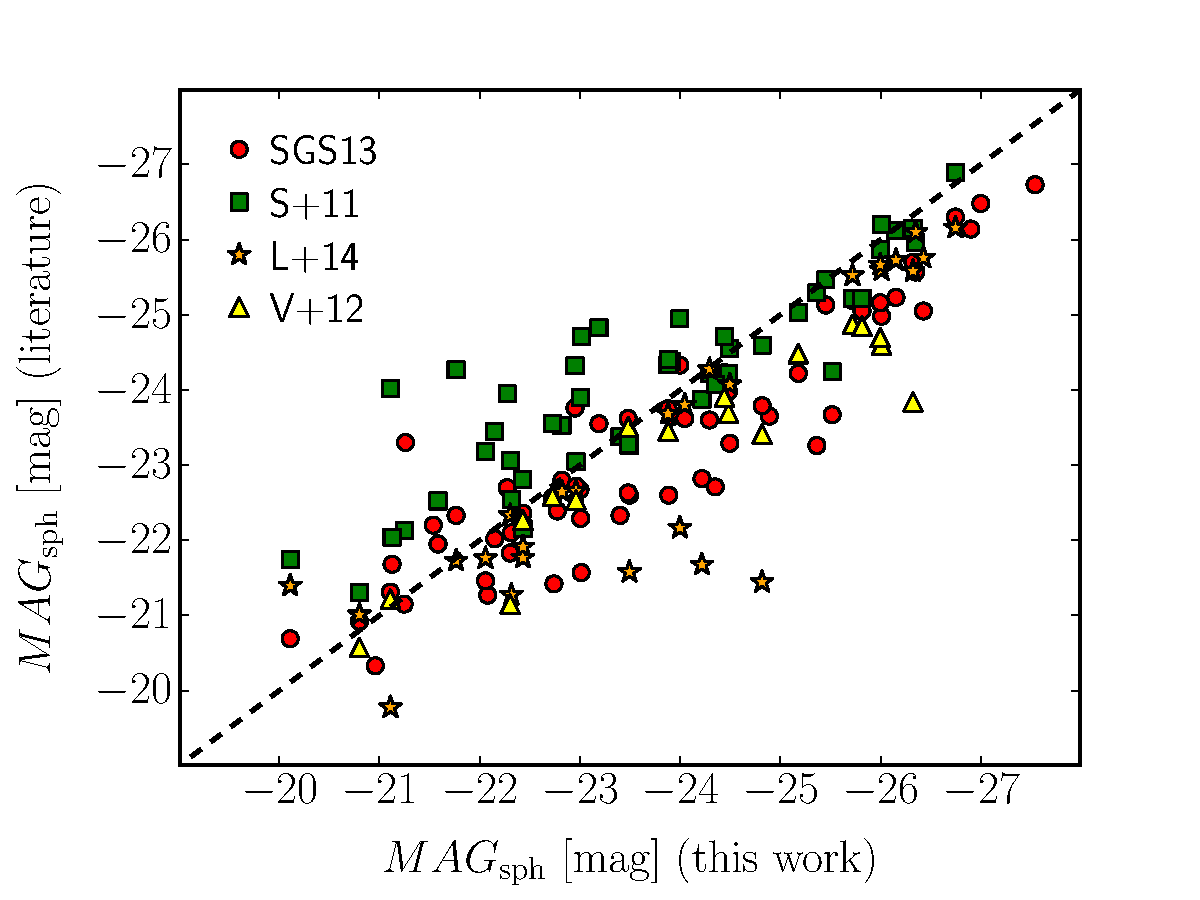
\includegraphics[width=\columnwidth]{images/mag_lit_vs_mag_my.pdf}
%\caption{}
%\label{fig:}
%\end{center}
%\end{figure}


\section{Analysis}
\label{sec:anal}

\begin{figure}[h]
\begin{center}
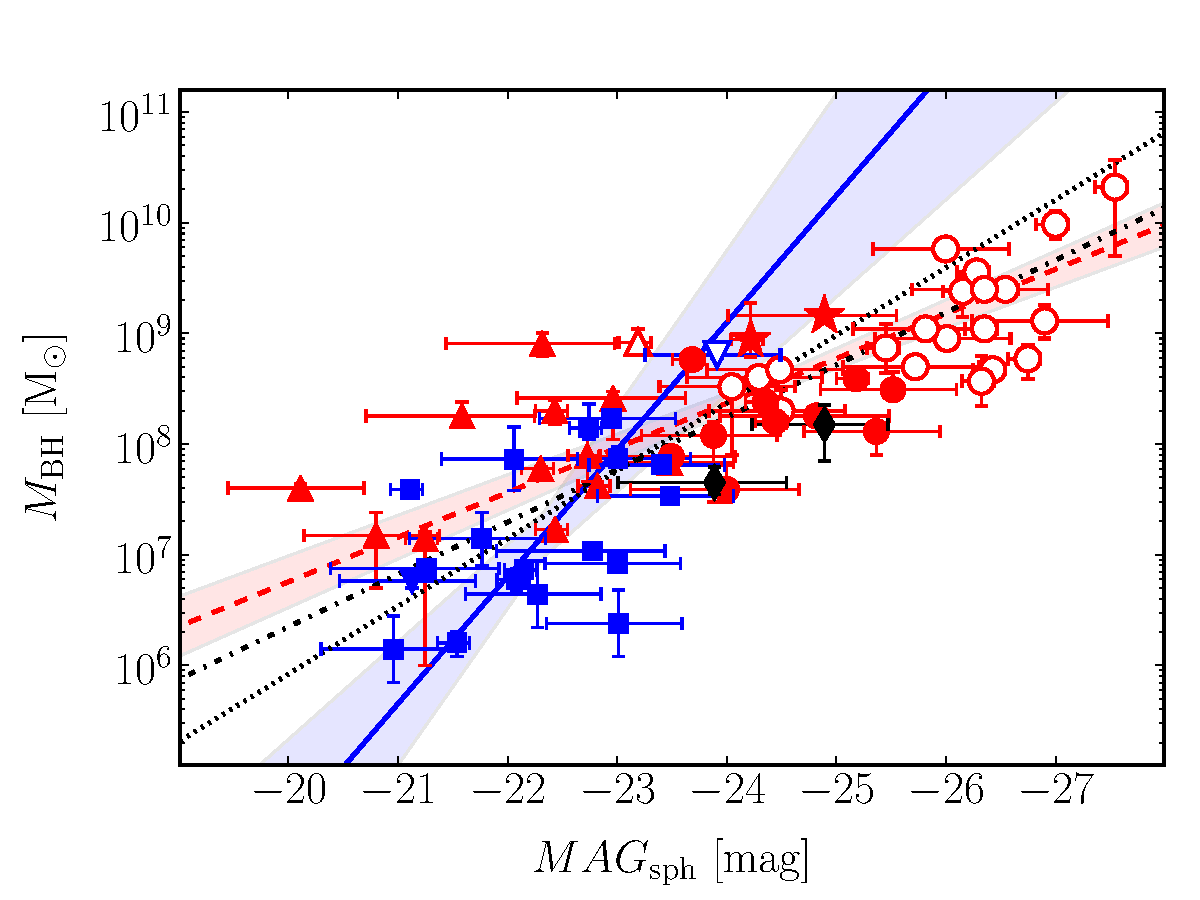
\includegraphics[width=\columnwidth]{images/mbh_vs_mag_sph.pdf}
\caption{Black hole mass against $3.6\rm~\mu m$ spheroid absolute magnitude. 
Symbols are coded according to the galaxy morphological type: red circle = elliptical, red star = elliptical/lenticular, 
red upward triangle = lenticular, blue downward triangle = lenticular/spiral, blue square = spiral, black diamond = merger. 
Empty symbols represent core-S\'ersic spheroids, whereas filled symbols are used for S\'ersic spheroids. 
The red dashed line indicates the BCES bisector linear regression for early-type galaxies (ellipticals+lenticulars), 
with the red shaded area denoting its $1\sigma$ uncertainty. 
The blue solid line shows the BCES bisector linear regression for spiral galaxies, 
with the blue shaded area denoting its $1\sigma$ uncertainty. 
The black dashed-dotted and dotted lines represent the BCES bisector linear regressions for core-S\'ersic and S\'ersic spheroids, respectively.}
\label{fig:mbhmagsph}
\end{center}
\end{figure}

\begin{figure}[h]
\begin{center}
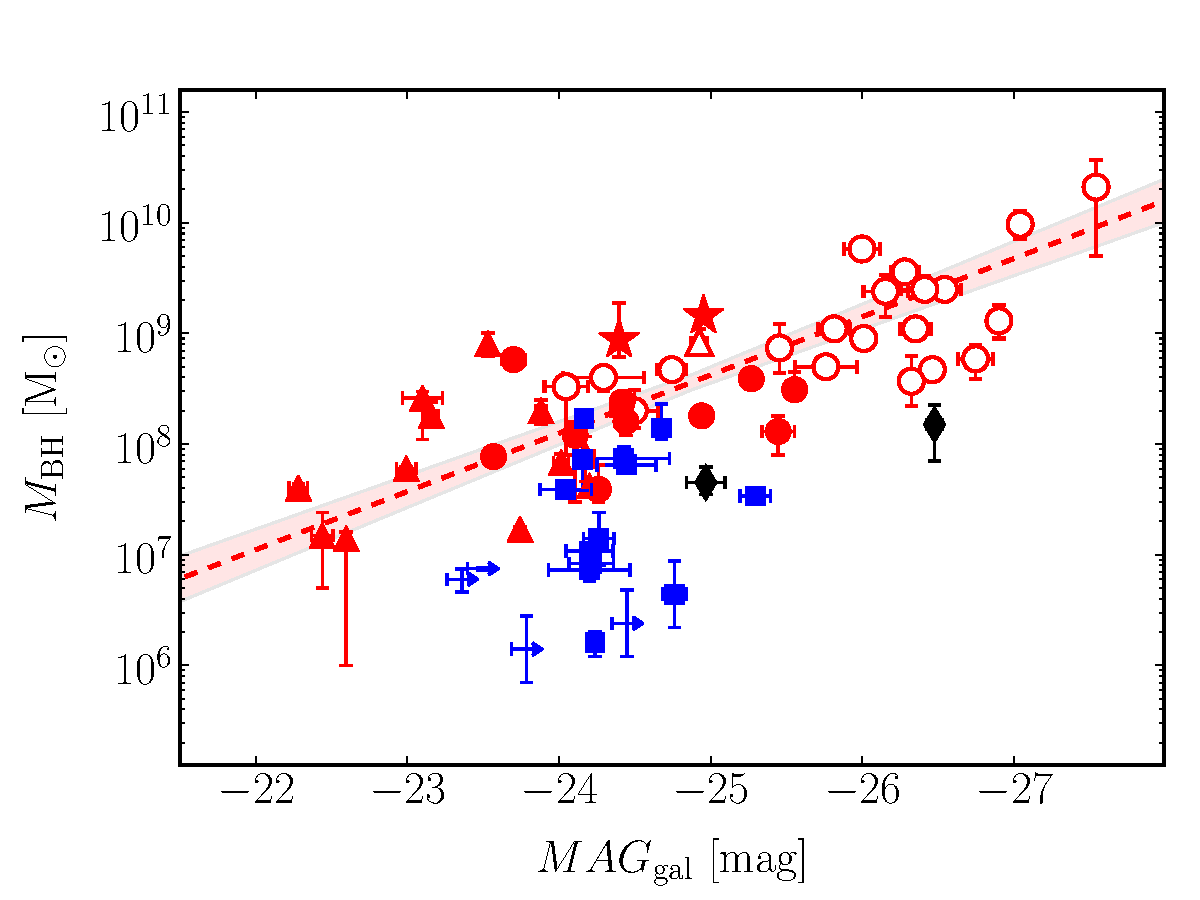
\includegraphics[width=\columnwidth]{images/mbh_vs_mag_tot.pdf}
\caption{Black hole mass against $3.6\rm~\mu m$ galaxy absolute magnitude. 
Symbols are coded as in Figure \ref{fig:mbhmagsph}.
Four spiral galaxies had their magnitudes overestimated and are shown as upper limits. 
}
\label{fig:}
\end{center}
\end{figure}



\begin{figure}[h]
\begin{center}
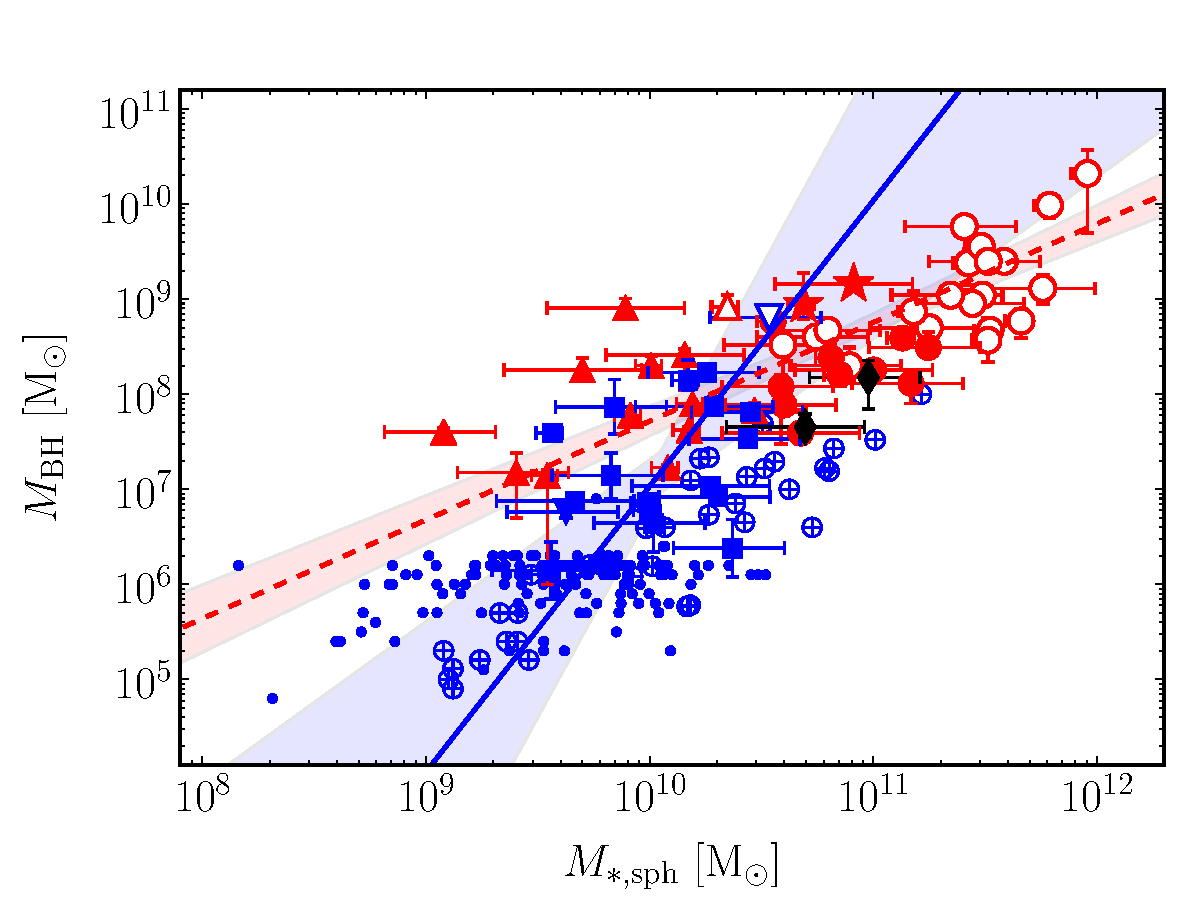
\includegraphics[width=\columnwidth]{images/mbh_vs_mass_sph_agn.pdf}
\caption{Black hole mass against spheroid stellar mass. 
Symbols are coded as in Figure \ref{fig:mbhmagsph}, 
with the addition of the blue dots representing {\bf the AGN sample Jiang}, 
and the blue crossed circles denoting {\bf the other AGNs}.
The red dashed line indicates the BCES bisector linear regression for early-type galaxies (ellipticals+lenticulars), 
with the red shaded area denoting its $1\sigma$ uncertainty. 
The blue solid line shows the BCES bisector linear regression for spiral galaxies, 
with the blue shaded area denoting its $1\sigma$ uncertainty. }
\label{fig:mbhmasssph}
\end{center}
\end{figure}




\begin{table*}
\centering
\caption{Linear regression analysis.}
\begin{tabular}{llccccc}
\hline
\hline
{\bf Subsample (size)} & {\bf Regression} & $\boldsymbol \alpha$ & $\boldsymbol \beta$ & $\boldsymbol X_0$ & $\boldsymbol \epsilon$ & $\boldsymbol \Delta$ \\ 
\hline 
\\
 & \multicolumn{6}{c}{$\log[M_{\rm BH}/{\rm M_\odot}] = \alpha + \beta[(MAG_{\rm sph} - X_0)/{\rm mag}]$} \\ [0.5em]
Core-S\'ersic (22) & BCES OLS$(Y|X)$   & $9.06 \pm 0.09$ & $-0.3  \pm 0.1$  & $-25.73$ & $-$    & $0.42$ \\ 
                   & BCES OLS$(X|Y)$   & $9.1  \pm 0.1$  & $-0.6  \pm 0.1$  & $-25.73$ & $-$    & $0.61$ \\
                   & BCES Bisector     & $9.1  \pm 0.1$  & $-0.47 \pm 0.08$ & $-25.73$ & $-$    & $0.48$ \\
                   & FITEXY OLS$(Y|X)$ & $9.06^{+0.09}_{-0.08}$ & $-0.26^{+0.07}_{-0.08}$ & $-25.73$ & $0.37$ & $0.42$ \\
                   & FITEXY OLS$(X|Y)$ & $9.0^{+0.1}_{-0.1}$ & $-0.7^{+0.2}_{-0.3}$ & $-25.73$ & $0.85$ & $0.67$ \\
                   & FITEXY Bisector   & $9.0^{+0.1}_{-0.1}$ & $-0.5^{+0.1}_{-0.2}$ & $-25.73$ & $-$    & $0.48$ \\

S\'ersic (44) & BCES OLS$(Y|X)$   & $7.71 \pm 0.09$ & $-0.41 \pm 0.08$ & $-22.92$ & $-$    & $0.61$ \\
              & BCES OLS$(X|Y)$   & $7.7  \pm 0.1$  & $-0.9  \pm 0.2 $ & $-22.92$ & $-$    & $0.93$ \\
              & BCES Bisector     & $7.7  \pm 0.1$  & $-0.61 \pm 0.08$ & $-22.92$ & $-$    & $0.71$ \\
              & FITEXY OLS$(Y|X)$ & $7.72^{+0.08}_{-0.08}$ & ${-0.41}^{+0.07}_{-0.07}$ & $-22.92$ & $0.54$ & $0.61$ \\
              & FITEXY OLS$(X|Y)$ & $7.7^{+0.1}_{-0.1}$ & $-0.9^{+0.1}_{-0.2}$ & $-22.92$ & $0.89$ & $0.93$ \\
              & FITEXY Bisector   & $7.7^{+0.1}_{-0.1}$ & $-0.61^{+0.09}_{-0.12}$ & $-22.92$ & $-$	& $0.71$ \\

%Ellipticals (E) (30)   & BCES OLS$(Y|X)$   & $8.80 \pm 0.07$ & $-0.53 \pm 0.09$ & $-25.45$ & $-$    & $0.42$ \\
% 		       & BCES OLS$(X|Y)$   & $8.80 \pm 0.08$ & $-0.66 \pm 0.07$ & $-25.45$ & $-$    & $0.48$ \\
% 		       & BCES Bisector     & $8.80 \pm 0.08$ & $-0.59 \pm 0.07$ & $-25.45$ & $-$    & $0.44$ \\
% 		       & FITEXY OLS$(Y|X)$ & $8.81^{+0.07}_{-0.07}$ & $-0.44^{+0.06}_{-0.07}$ & $-25.45$ & $0.33$     & $0.40$ \\
% 		       & FITEXY OLS$(X|Y)$ & $8.78^{+0.09}_{-0.09}$ & $-0.7^{+0.1}_{-0.1}$    & $-25.45$ & $0.60$     & $0.50$\\
% 		       & FITEXY Bisector   & $8.80^{+0.08}_{-0.08}$ & $-0.56^{+0.08}_{-0.10}$ & $-25.45$ & $-$        & $0.43$ \\
%
%Lenticulars (S0) (13)  & BCES OLS$(Y|X)$   & $7.9 \pm 0.1$ & $-0.4 \pm 0.2$ & $-22.19$ & $-$    & $0.56$ \\
% 		       & BCES OLS$(X|Y)$   & $7.9 \pm 0.3$ & $-1.1 \pm 0.5$ & $-22.19$ & $-$    & $1.01$ \\
% 		       & BCES Bisector     & $7.9 \pm 0.2$ & $-0.7 \pm 0.2$ & $-22.19$ & $-$    & $0.69$ \\
% 		       & FITEXY OLS$(Y|X)$ & $7.9^{+0.2}_{-0.1}$ & $-0.3^{+0.2}_{-0.2}$ & $-22.19$ & $0.51$     & $0.56$ \\
% 		       & FITEXY OLS$(X|Y)$ & $7.8^{+0.3}_{-0.4}$ & $-1.3^{+0.4}_{-1.3}$ & $-22.19$ & $0.71$     & $1.20$\\
% 		       & FITEXY Bisector   & $7.9^{+0.2}_{-0.3}$ & $-0.7^{+0.3}_{-0.4}$ & $-22.19$ & $-$        & $0.71$ \\
%
Early-type (E+S0) (45) & BCES OLS$(Y|X)$   & $8.56 \pm 0.07$ & $-0.33 \pm 0.04$ & $-24.47$ & $-$    & $0.46$ \\
 		       & BCES OLS$(X|Y)$   & $8.56 \pm 0.08$ & $-0.48 \pm 0.05$ & $-24.47$ & $-$    & $0.55$ \\
 		       & BCES Bisector     & $8.56 \pm 0.07$ & $-0.40 \pm 0.04$ & $-24.47$ & $-$    & $0.49$ \\
 		       & FITEXY OLS$(Y|X)$ & $8.56^{+0.06}_{-0.06}$ & $-0.32^{+0.03}_{-0.04}$ & $-24.47$ & $0.40$ & $0.46$ \\
 		       & FITEXY OLS$(X|Y)$ & $8.54^{+0.08}_{-0.08}$ & $-0.49^{+0.05}_{-0.06}$ & $-24.47$ & $1.00$ & $0.57$\\
 		       & FITEXY Bisector   & $8.55^{+0.07}_{-0.07}$ & $-0.41^{+0.04}_{-0.05}$ & $-24.47$ & $-$    & $0.49$ \\

Late-type (S) (17) & BCES OLS$(Y|X)$   & $7.2 \pm 0.2$ & $-0.8 \pm 0.4$ & $-22.33$ & $-$    & $0.70$ \\
 		   & BCES OLS$(X|Y)$   & $7.2 \pm 0.3$ & $-1.7 \pm 0.7$ & $-22.33$ & $-$    & $1.26$ \\
 		   & BCES Bisector     & $7.2 \pm 0.2$ & $-1.1 \pm 0.3$ & $-22.33$ & $-$    & $0.88$ \\
 		   & FITEXY OLS$(Y|X)$ & $7.2^{+0.1}_{-0.1}$ & $-0.5^{+0.2}_{-0.2}$ & $-22.33$ & $0.54$ & $0.63$ \\
 		   & FITEXY OLS$(X|Y)$ & $7.4^{+0.5}_{-0.3}$ & $-2.0^{+0.7}_{-2.3}$ & $-22.33$ & $0.54$ & $1.51$ \\
 		   & FITEXY Bisector   & $7.3^{+0.4}_{-0.3}$ & $-1.0^{+0.3}_{-0.5}$ & $-22.33$ & $-$    & $0.82$ \\
\hline 
\\
 & \multicolumn{6}{c}{$\log[M_{\rm BH}/{\rm M_\odot}] = \alpha + \beta[(MAG_{\rm gal} - X_0)/{\rm mag}]$} \\ [0.5em]
Early-type (E+S0) (45) & BCES OLS$(Y|X)$   & $8.56 \pm 0.06$ & $-0.43 \pm 0.05$ & $$ & $-$ & $0.4487$ \\
 		       & BCES OLS$(X|Y)$   & $8.56 \pm 0.08$ & $-0.63 \pm 0.05$ & $$ & $-$ & $0.5329$ \\
 		       & BCES Bisector     & $8.56 \pm 0.07$ & $-0.53 \pm 0.04$ & $$ & $-$ & $0.4713$ \\
 		       & FITEXY OLS$(Y|X)$ & $$ & $$ & $$ & $$ & $$ \\
 		       & FITEXY OLS$(X|Y)$ & $$ & $$ & $$ & $$ & $$ \\
 		       & FITEXY Bisector   & $$ & $$ & $$ & $-$    & $$ \\
		   
		  
\hline 
\hline
\end{tabular}
\label{tab:lreg} 
\end{table*}

\section{Results}
\label{sec:res}

compare scatter mbh-msph and mbh-mgal for early types

if 2 overmassive bhs removed, what happens?


\section{Conclusions}
\label{sec:concl}



\acknowledgments
%{\bf marconi, sani, hunt...}
%GS warmly thanks Chieng Peng, Peter Erwin, Luca Cortese, Elisabete Lima Da Cunha and Gonzalo Diaz 
%for useful discussion. \\
This research was supported by Australian Research Council funding through grants
DP110103509 and FT110100263.
This work is based on observations made with the IRAC instrument \citep{fazio2004IRAC} 
on-board the Spitzer Space Telescope, 
which is operated by the Jet Propulsion Laboratory, 
California Institute of Technology under a contract with NASA.
This research has made use of the GOLDMine database \citep{goldmine} and the NASA/IPAC Extragalactic Database (NED) 
which is operated by the Jet Propulsion Laboratory, California Institute of Technology, 
under contract with the National Aeronautics and Space Administration. 


\bibliography{/Users/gsavorgnan/Dropbox_notsync/giulia_e_basta/Literature/SMBHbibliography}


\clearpage


\end{document}

